\chapter{Architettura del Prodotto}\label{ArchitetturaDelProdotto}
L'architettura generale del software$_{\scaleto{G}{3pt}}$ \textit{Gathering-Detection-Platform} è un'architettura monolitica distribuita.
Si tratta di due file eseguibili, scritti in Python$_{\scaleto{G}{3pt}}$, che sono rispettivamente il modulo Acquisition e il modulo Prediction.
Il primo viene utilizzato per acquisire le informazione estrapolate dalle live webcams delle città, il secondo invece viene utilizzato per calcolare predizioni su periodi di tempo futuri, utilizzando il machine-learning$_{\scaleto{G}{3pt}}$.
Entrambi sono collegati ad un database, il quale serve per salvare ed esportare i dati in esso.
Il terzo, ed ultimo, modulo riguarda la web-app$_{\scaleto{G}{3pt}}$ vera e propria, che permette all'utente utilizzatore di visualizzare la heat-map$_{\scaleto{G}{3pt}}$ relativa alla città.

\section{Architettura modulo Acquisition}
\subsection{Diagramma dei Package}
\begin{figure}[!h]
  \begin{center}
    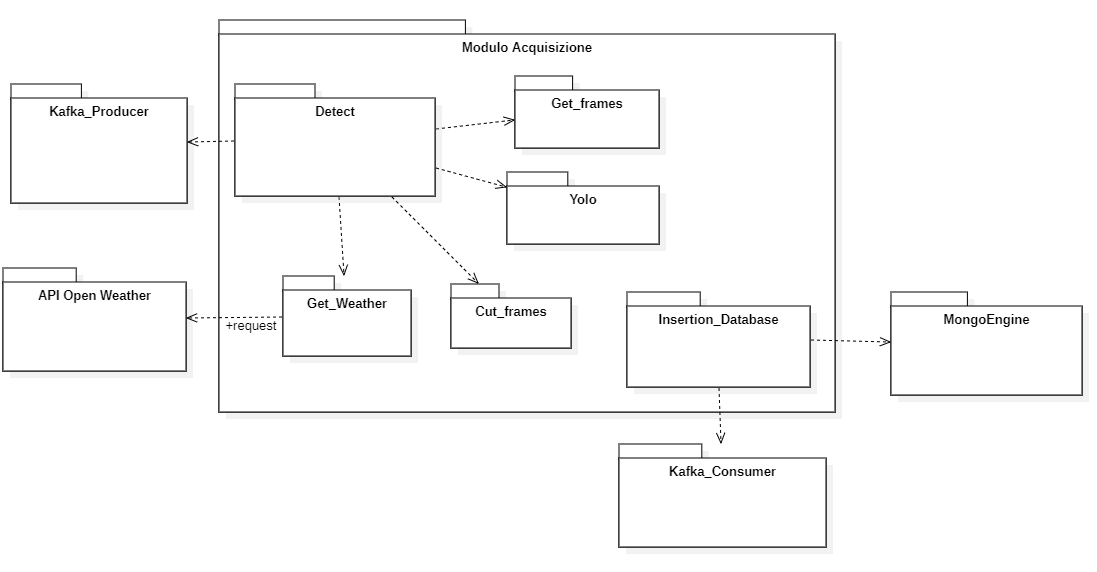
\includegraphics[width=1\linewidth]{../immagini/diag_PB/diag_pack_acqui.png}
    \caption{Diagramma dei package del modulo Acquisition}
  \end{center}
\end{figure}

\subsection{Diagrammi di attività}
\begin{figure}[!h]
  \begin{center}
    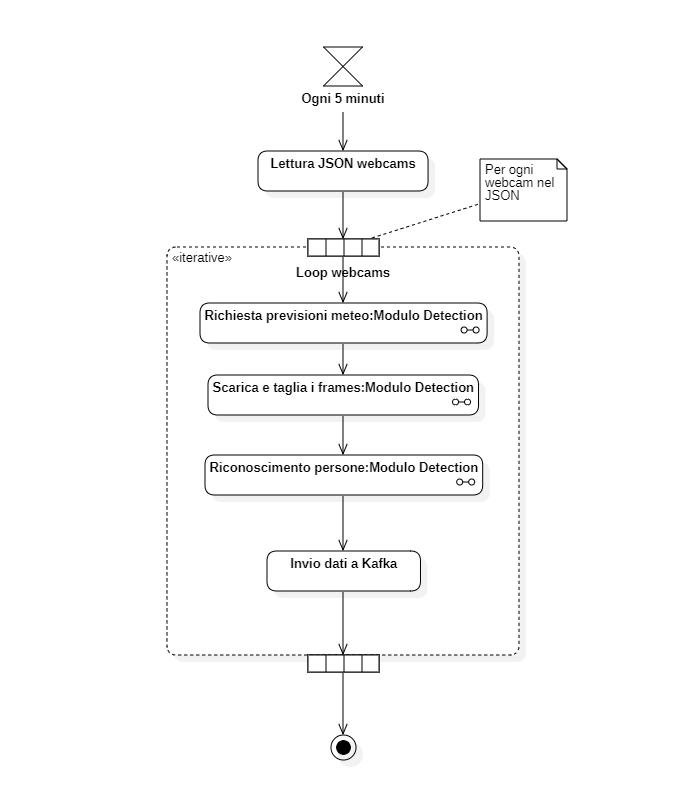
\includegraphics[width=1\linewidth]{../immagini/diag_PB/detection.png}
    \caption{Diagramma di attività dell'eseguibile Detection}
  \end{center}
\end{figure}
\begin{figure}[!h]
  \begin{center}
    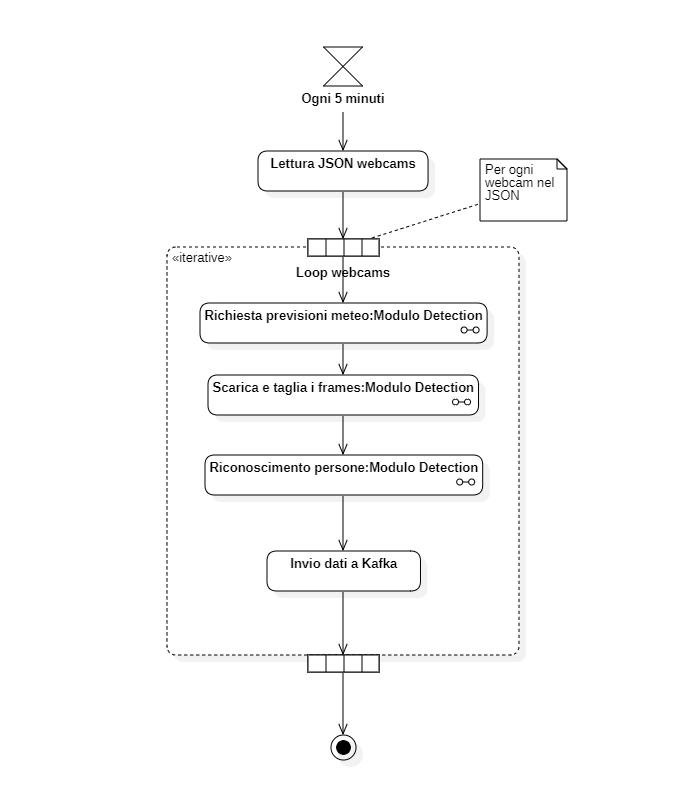
\includegraphics[width=1\linewidth]{../immagini/diag_PB/detection.png}
    \caption{Diagramma di sotto-attività dell'acquisizione delle previsioni meteo}
  \end{center}
\end{figure}
\begin{figure}[!h]
  \begin{center}
    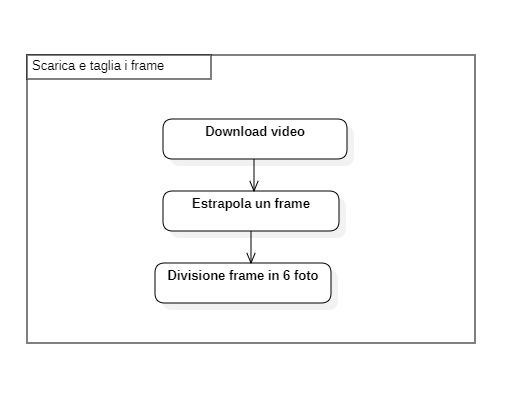
\includegraphics[width=1\linewidth]{../immagini/diag_PB/download_e_cut_frames.png}
    \caption{Diagramma di sotto-attività di download e taglio frame}
  \end{center}
\end{figure}
\begin{figure}[!h]
  \begin{center}
    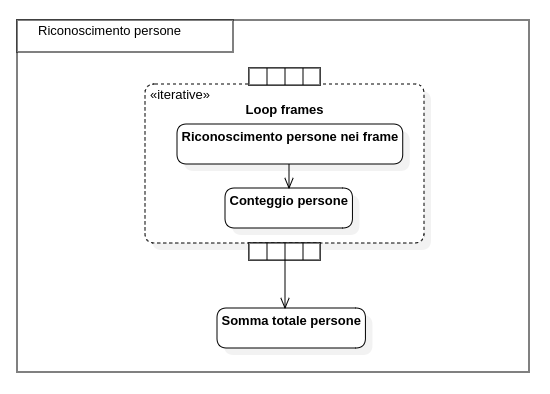
\includegraphics[width=1\linewidth]{../immagini/diag_PB/conta_persone.png}
    \caption{Diagramma di sotto-attività del conta persone}
  \end{center}
\end{figure}
\begin{figure}[!h]
  \begin{center}
    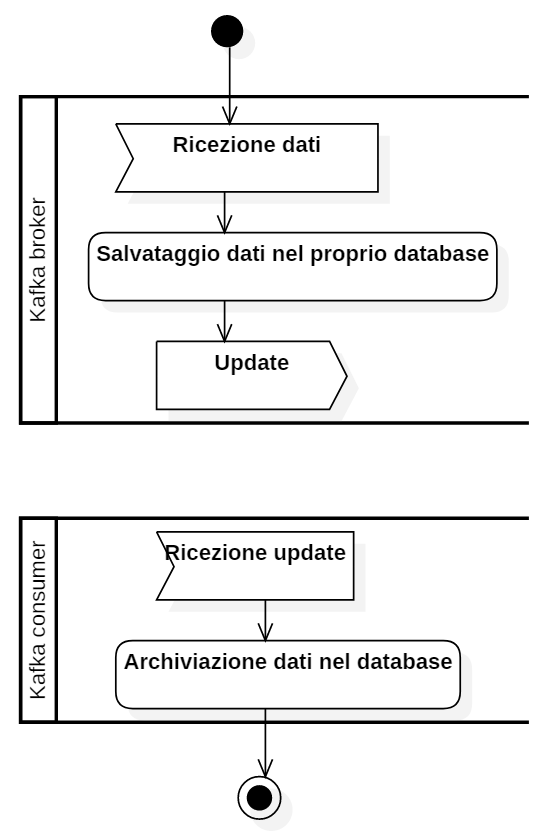
\includegraphics[width=1\linewidth]{../immagini/diag_PB/kafka.png}
    \caption{Diagramma di attività di Kafka}
  \end{center}
\end{figure}


\section{Architettura modulo Prediction}
\subsection{Diagramma dei package}
\begin{figure}[!h]
  \begin{center}
    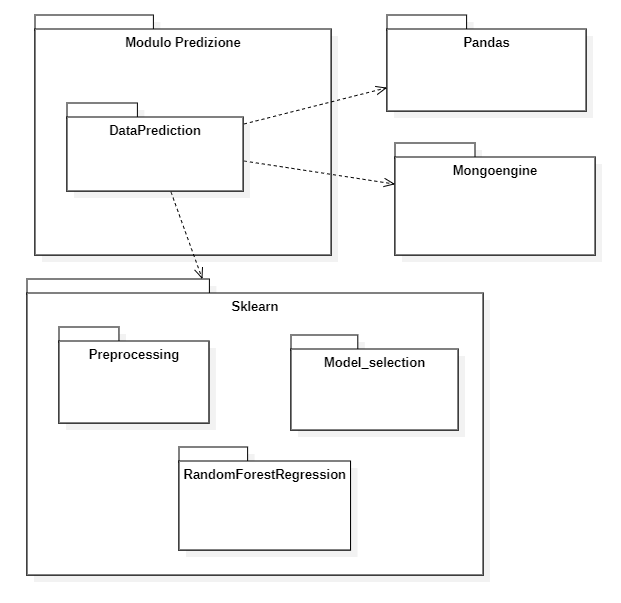
\includegraphics[width=1\linewidth]{../immagini/diag_PB/diag_pack_pred.png}
    \caption{Diagramma dei package del modulo Acquisition}
  \end{center}
\end{figure}

\subsection{Diagramma di attività}
\begin{figure}[!h]
  \begin{center}
    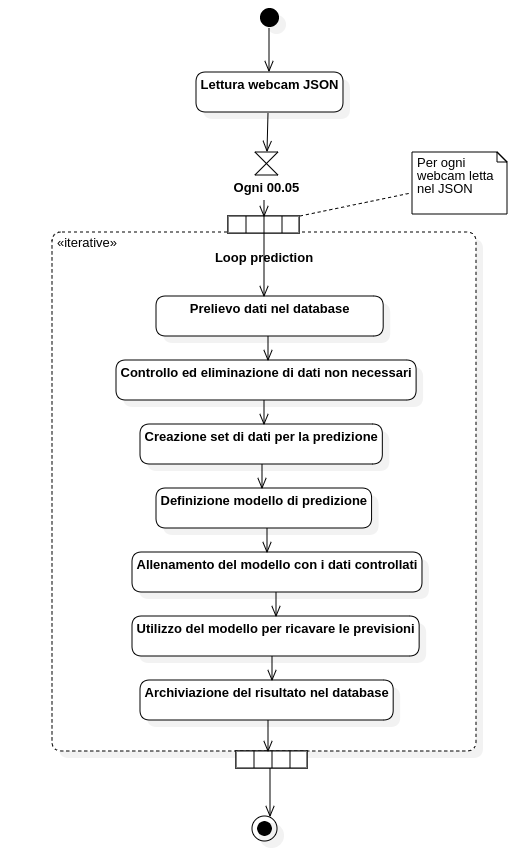
\includegraphics[width=1\linewidth]{../immagini/diag_PB/prediction_activity.png}
    \caption{Diagramma di attività dell'eseguibile Detection}
  \end{center}
\end{figure}



\section{Architettura modulo Web-app}
\subsection{Diagrammi dei package}
\begin{figure}[!h]
  \begin{center}
    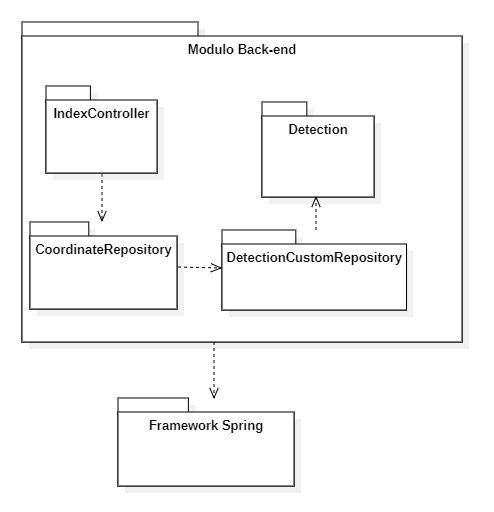
\includegraphics[width=1\linewidth]{../immagini/diag_PB/diag_pack_spring.png}
    \caption{Diagramma dei package di Spring}
  \end{center}
\end{figure}

\begin{figure}[!h]
  \begin{center}
    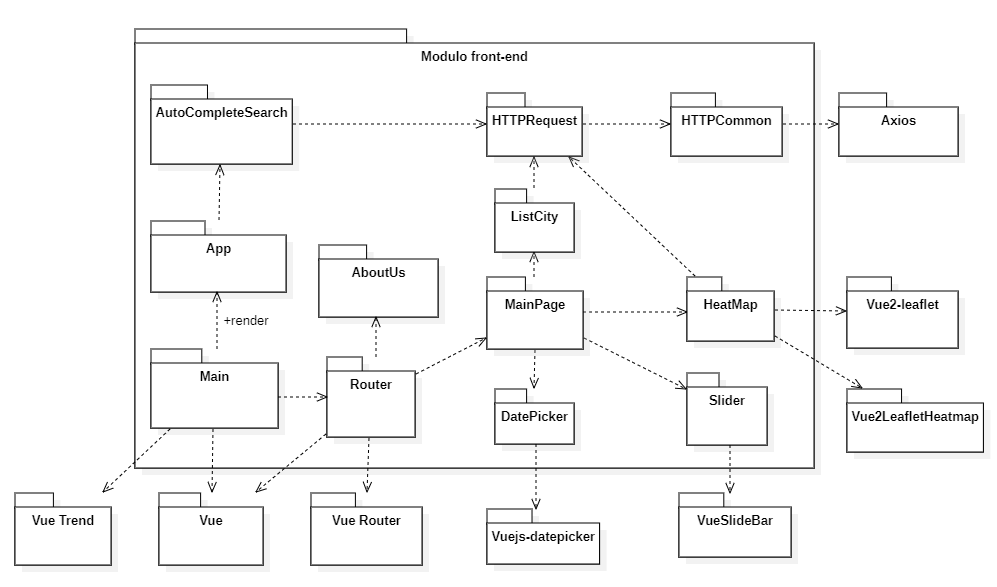
\includegraphics[width=1\linewidth]{../immagini/diag_PB/diag_pack_vue.png}
    \caption{Diagramma dei package del modulo Acquisition}
  \end{center}
\end{figure}

\subsection{Diagrammi delle classi}
\begin{figure}[!h]
  \begin{center}
    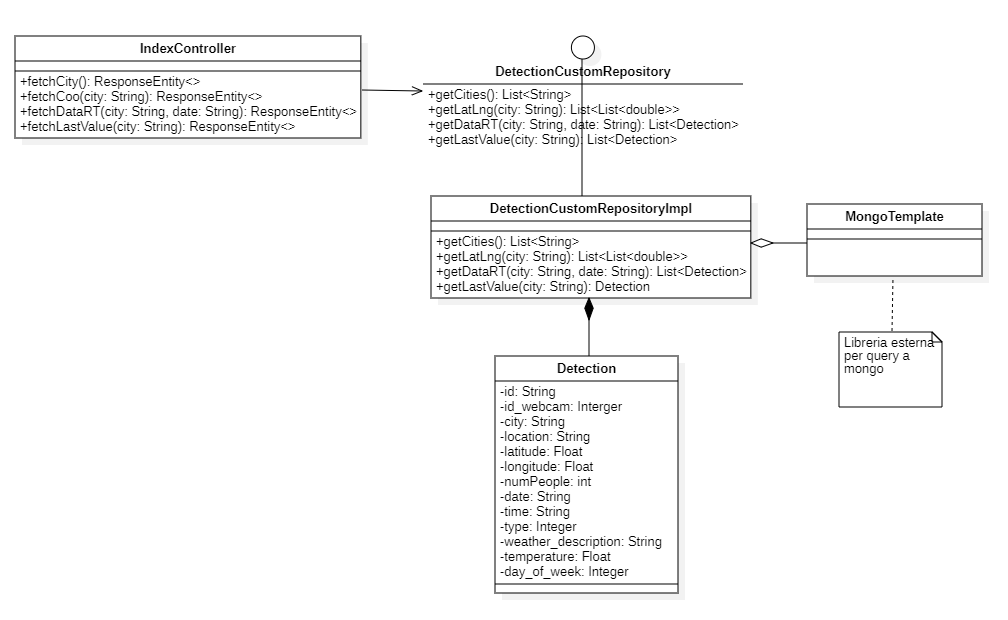
\includegraphics[width=1\linewidth]{../immagini/diag_PB/diag_class_spring.png}
    \caption{Diagramma delle classi di Spring}
  \end{center}
\end{figure}

\subsection{Diagramma di sequenza}
\begin{figure}[!h]
  \begin{center}
    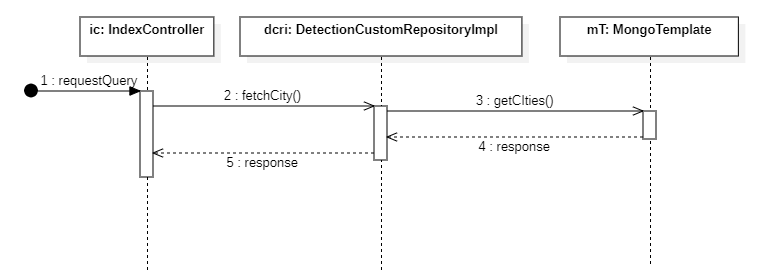
\includegraphics[width=1\linewidth]{../immagini/diag_PB/diag_seq_spring.png}
    \caption{Diagramma di sequenza di Spring}
  \end{center}
\end{figure}

\subsection{Diagramma di attività}
\begin{figure}[!h]
  \begin{center}
    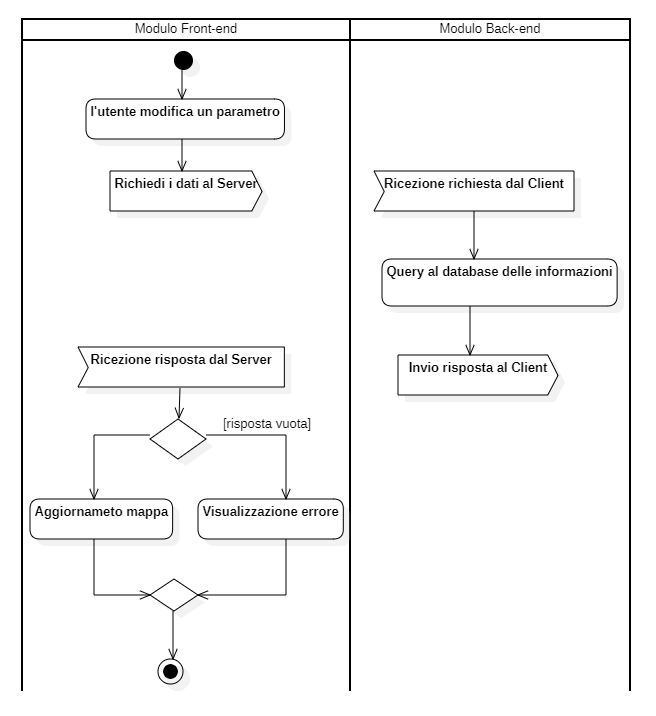
\includegraphics[width=1\linewidth]{../immagini/diag_PB/diag_act_front_back.png}
    \caption{Diagramma di attività del modulo Web-app}
  \end{center}
\end{figure}
